\documentclass{ctexart}
\usepackage{geometry}
\usepackage{hyperref}
\usepackage{amsmath}
\usepackage{float}
\usepackage{subfigure}
\usepackage{graphicx}
\title{基于虚拟仪器技术的电路综合实验报告}
\author{陈启钰\,\,2300011447}
\date{\today}
\begin{document}
	\maketitle
	\tableofcontents
	\section{第一次课}
	\subsection{电阻伏安曲线测量结果}
	第一次实验中,测得的电阻伏安特性曲线结果如下。
	\begin{figure}[H]
		\centering
		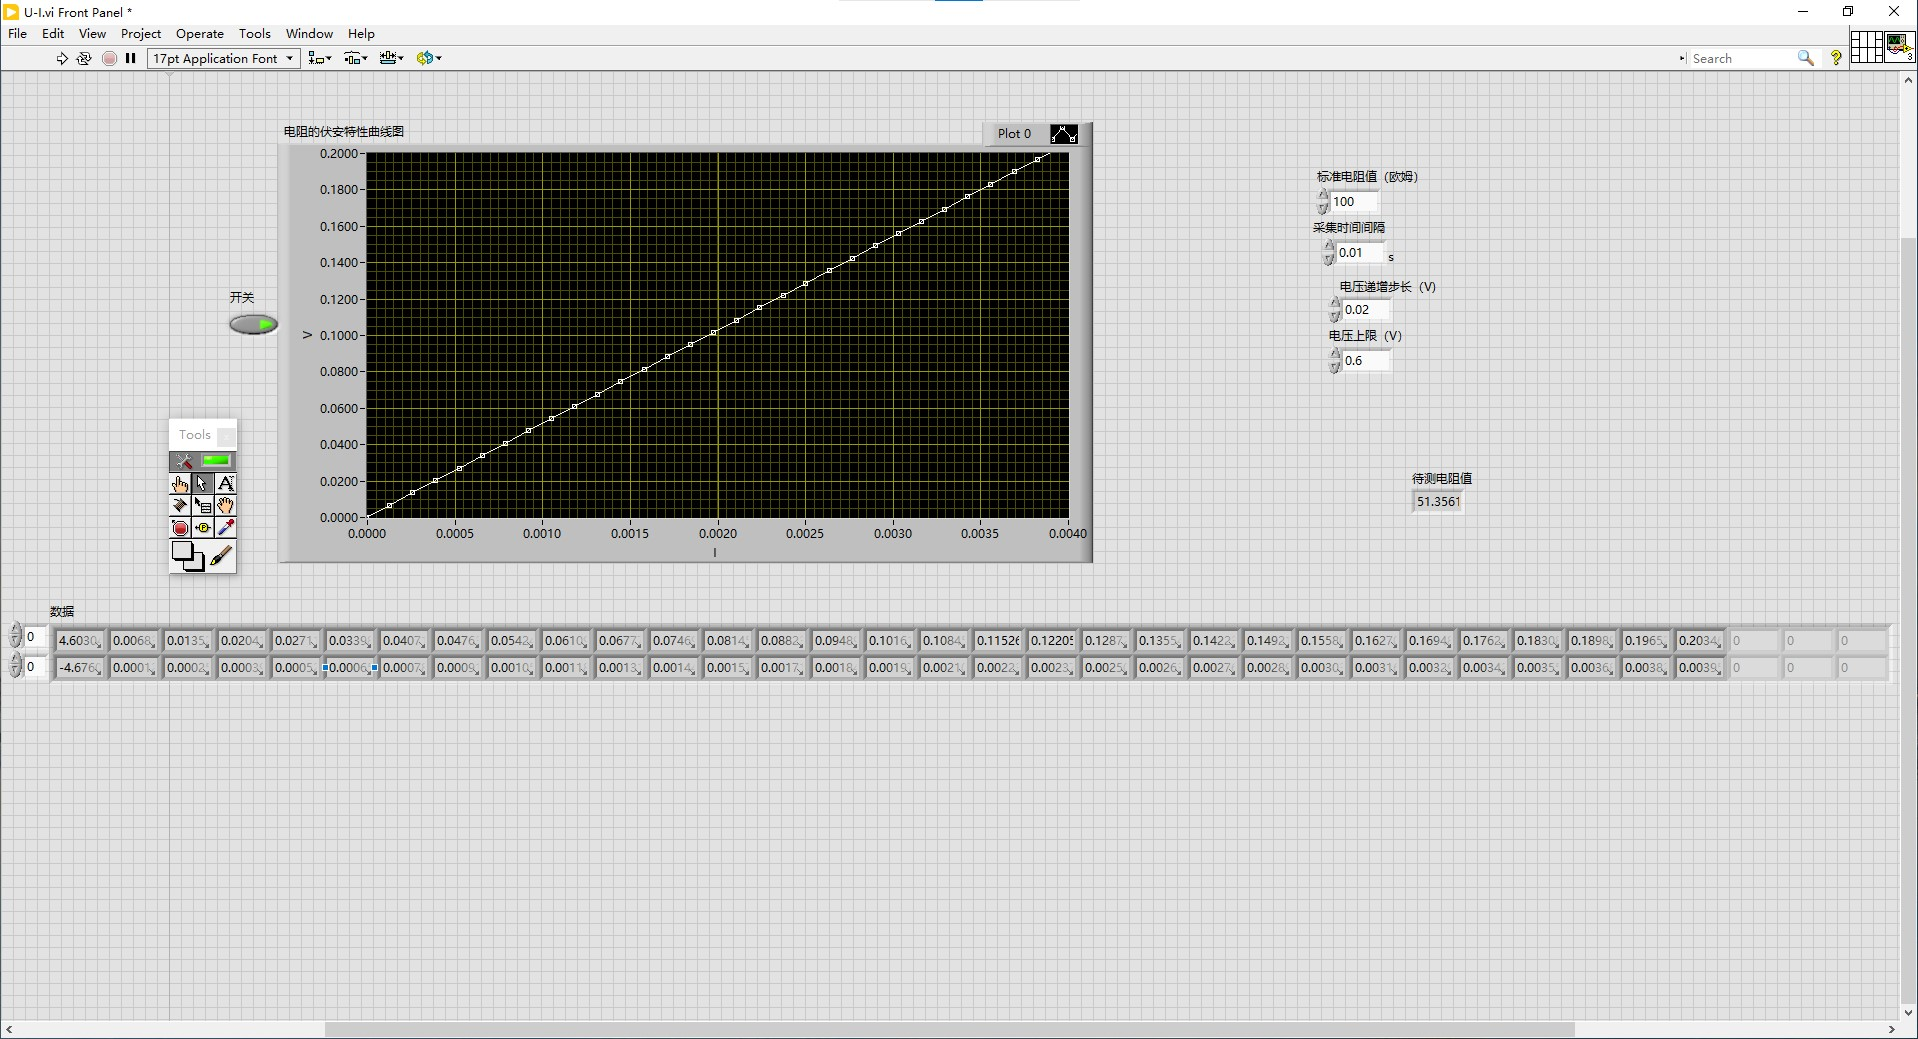
\includegraphics[width=\linewidth]{ui1.jpg}
	\end{figure}
	\begin{figure}[H]
		\centering
		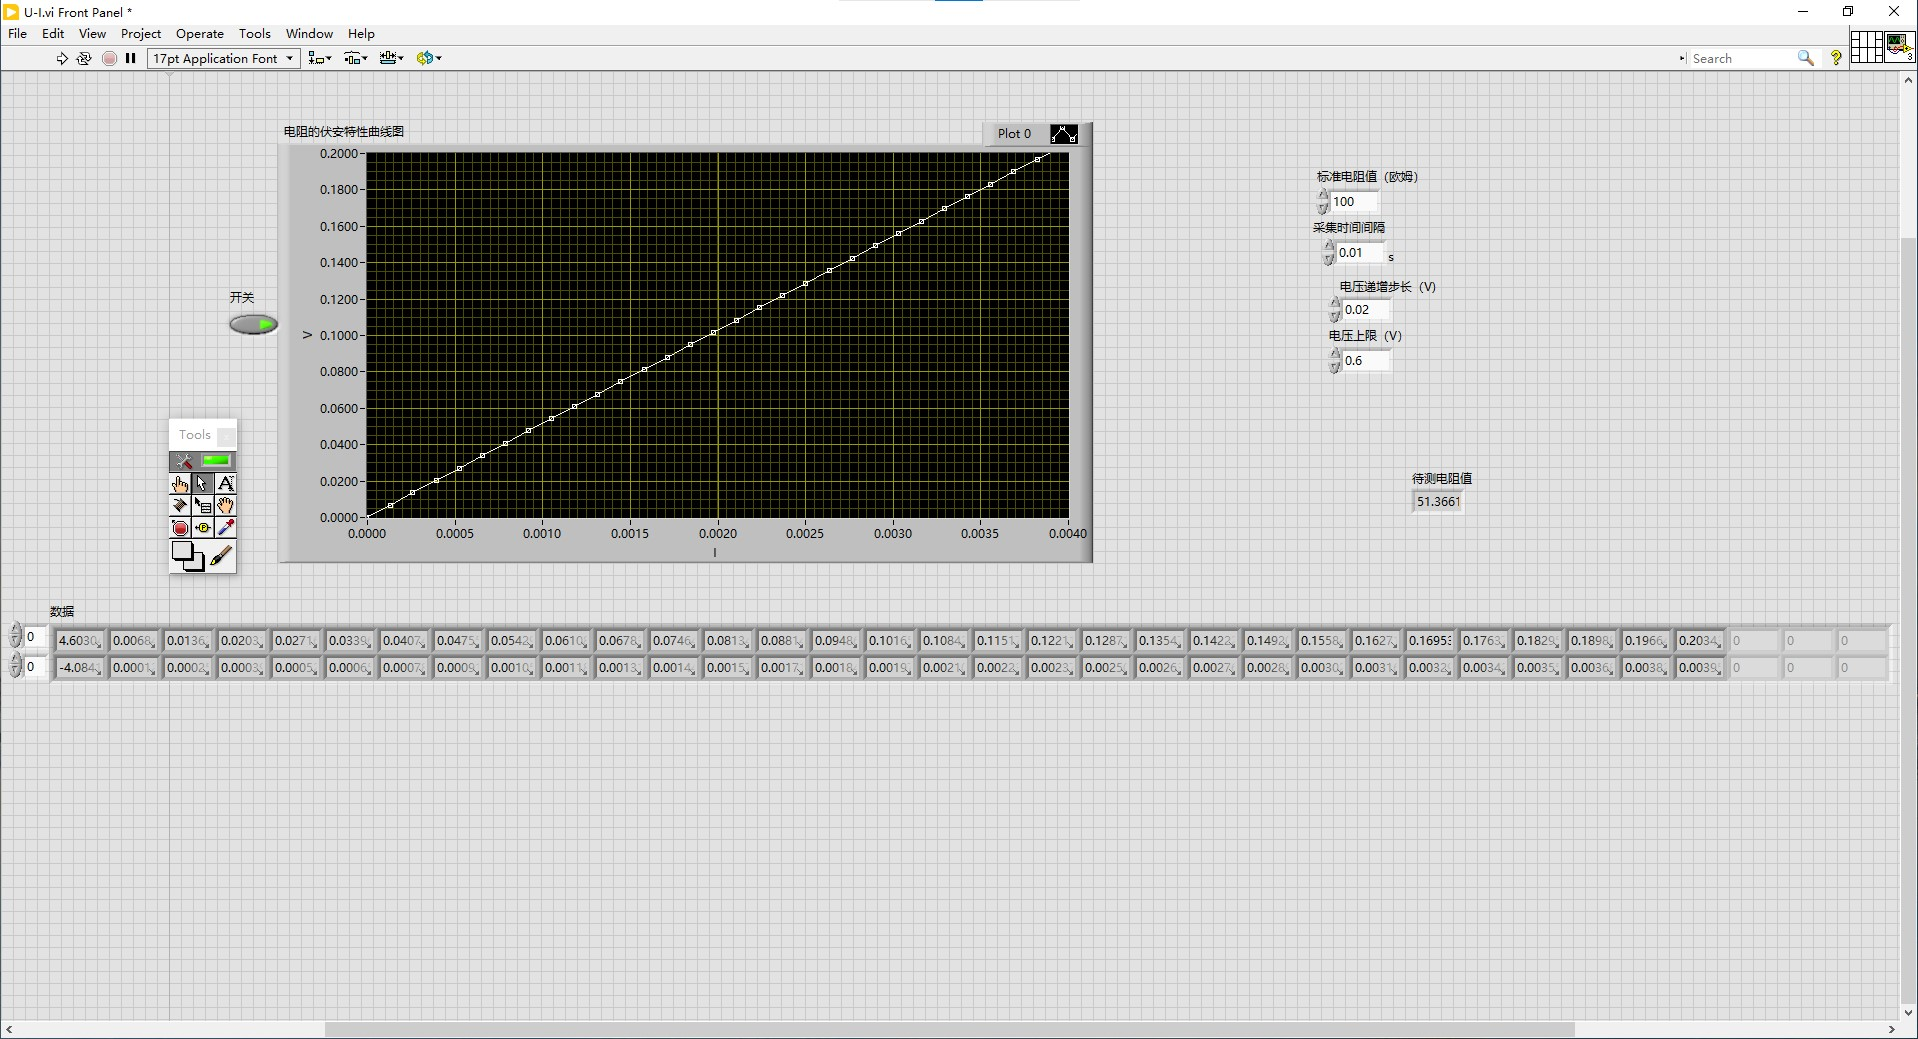
\includegraphics[width=\linewidth]{ui2.jpg}
	\end{figure}
	\begin{figure}[H]
		\centering
		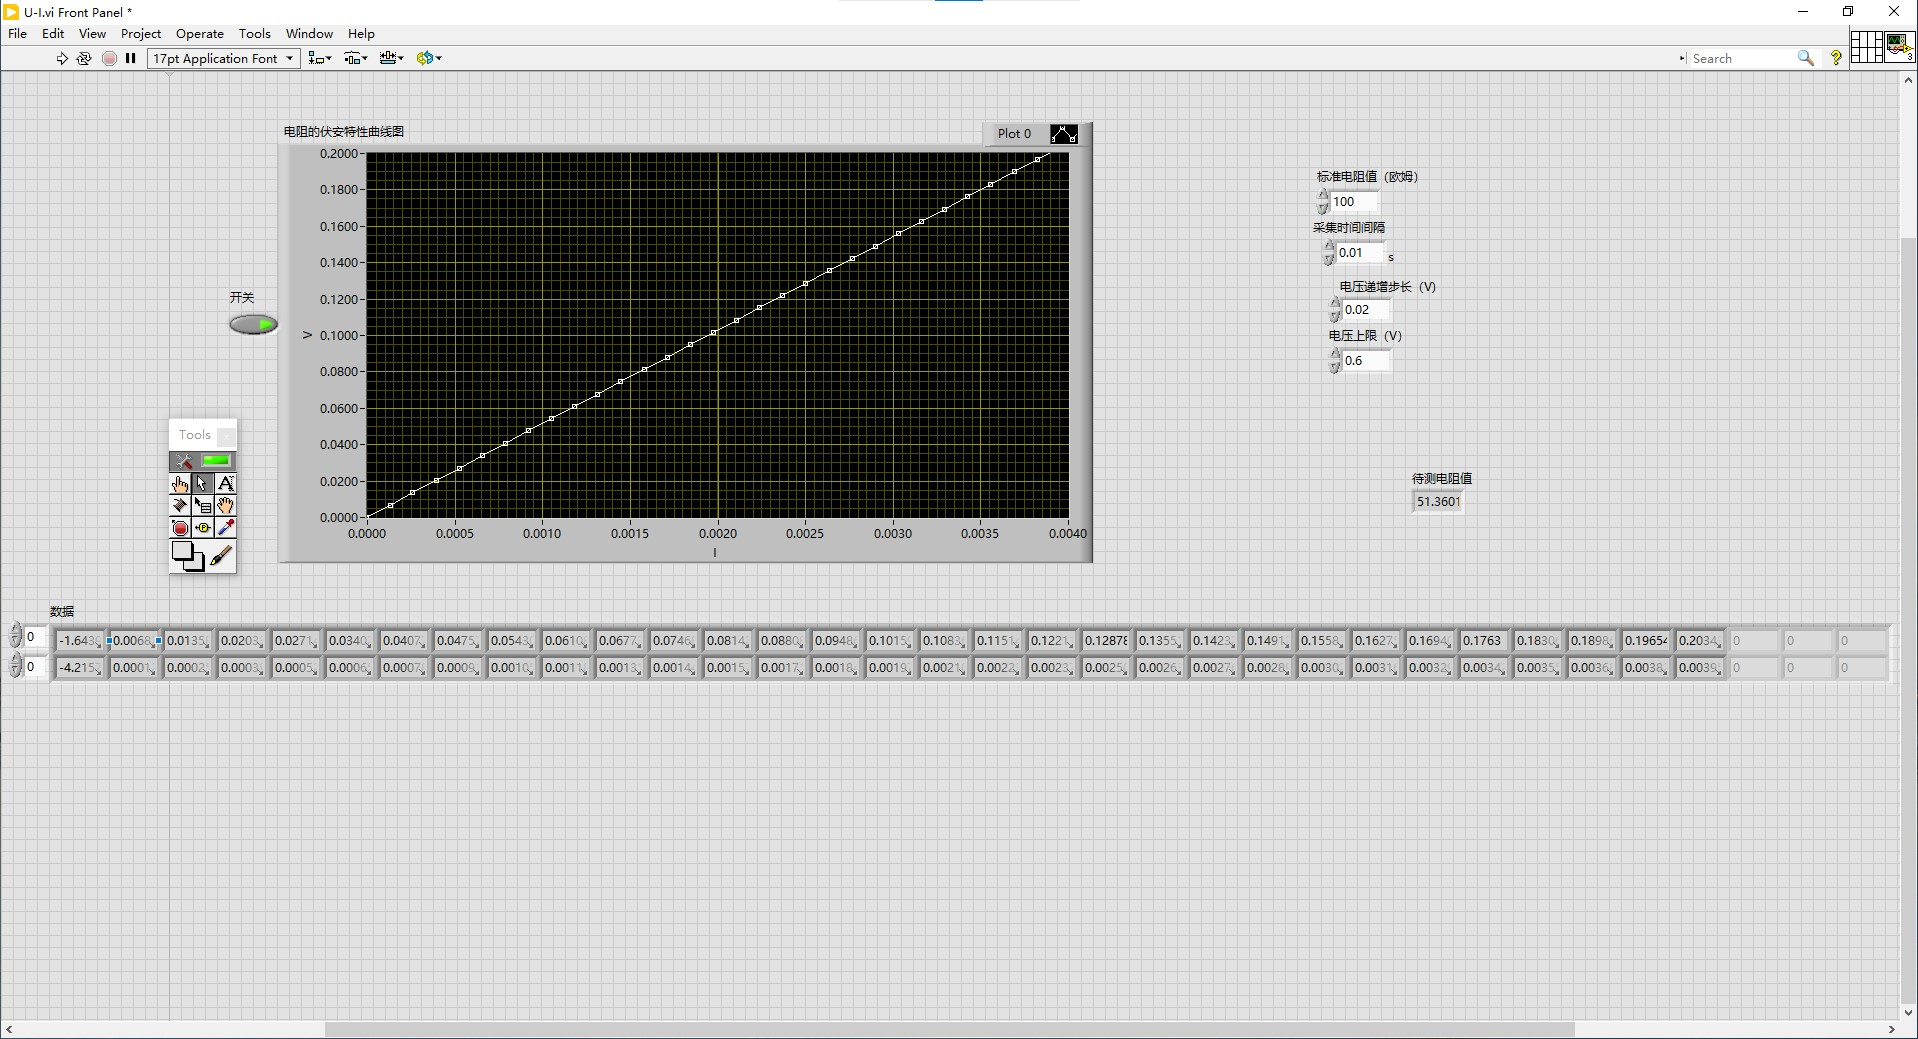
\includegraphics[width=\linewidth]{ui3.jpg}
		\caption{$50\Omega$电阻测量结果}
	\end{figure}
	\begin{figure}[H]
		\centering
		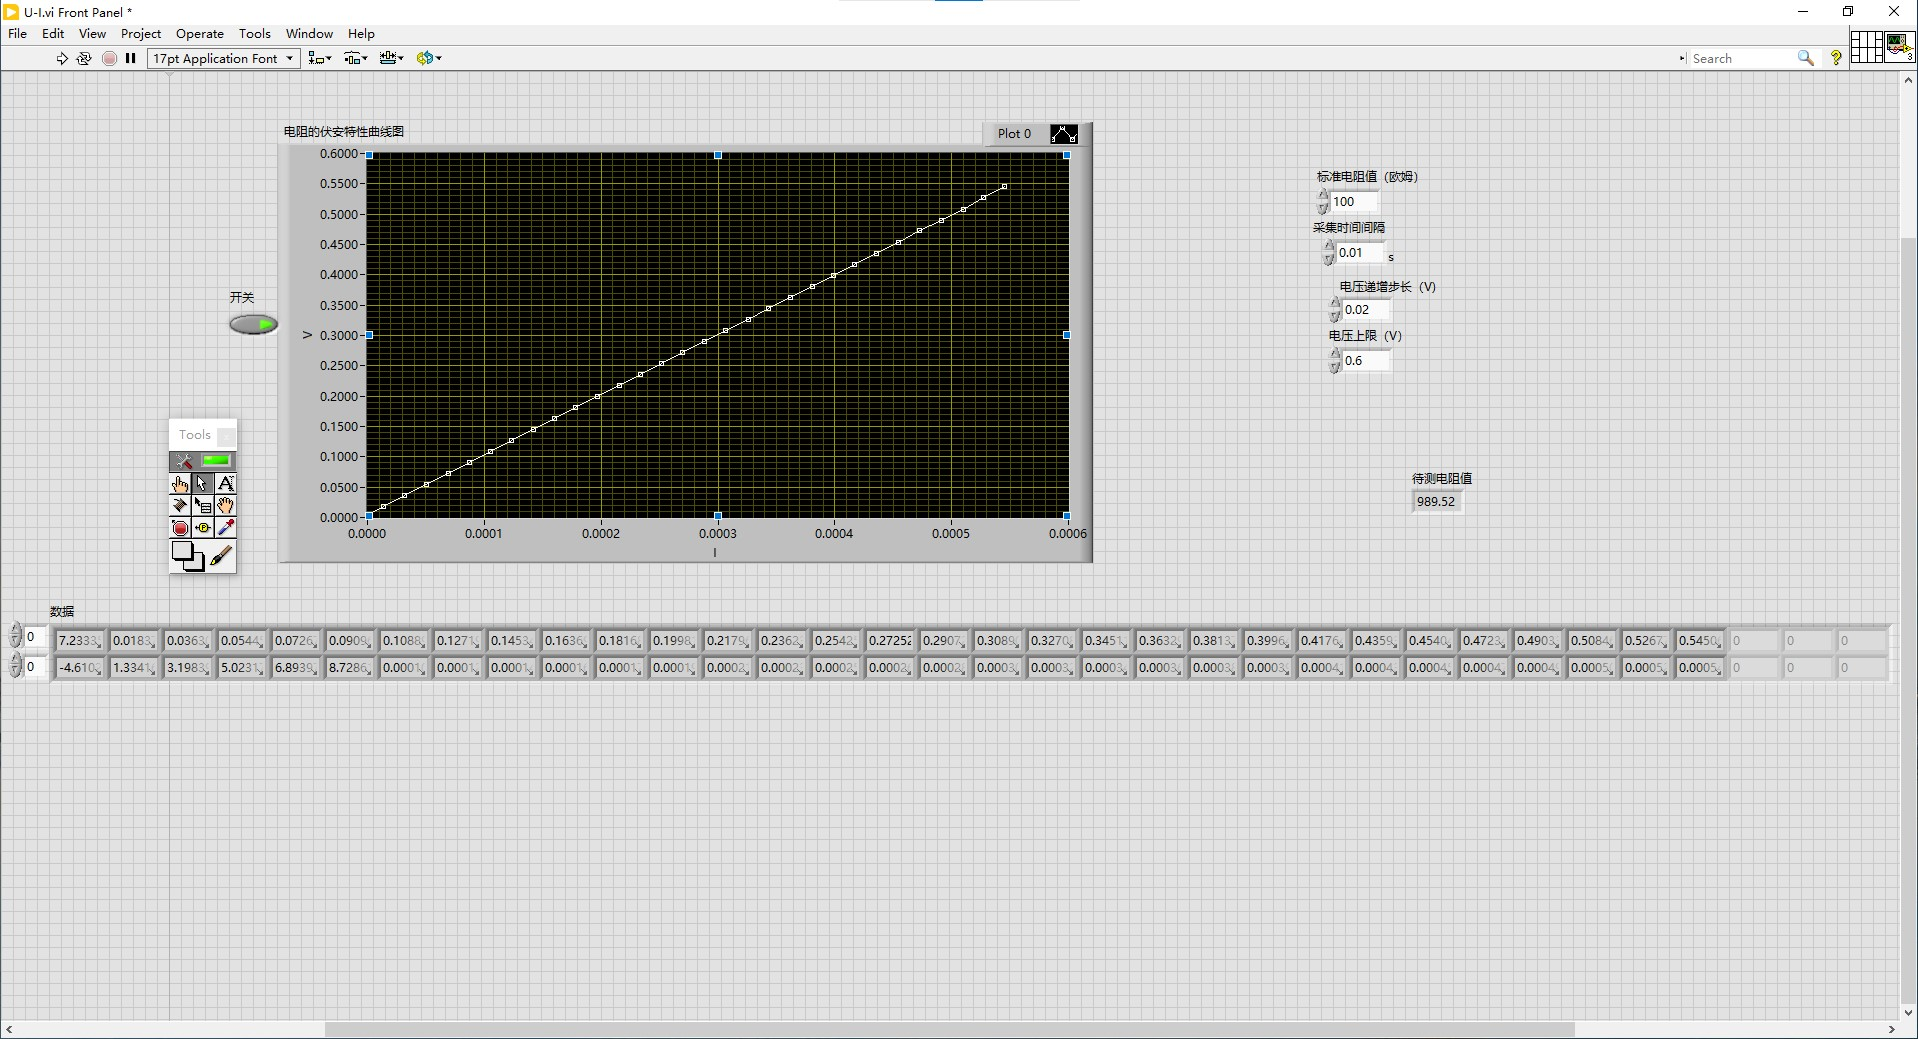
\includegraphics[width=\linewidth]{ui4.jpg}
	\end{figure}
	\begin{figure}[H]
		\centering
		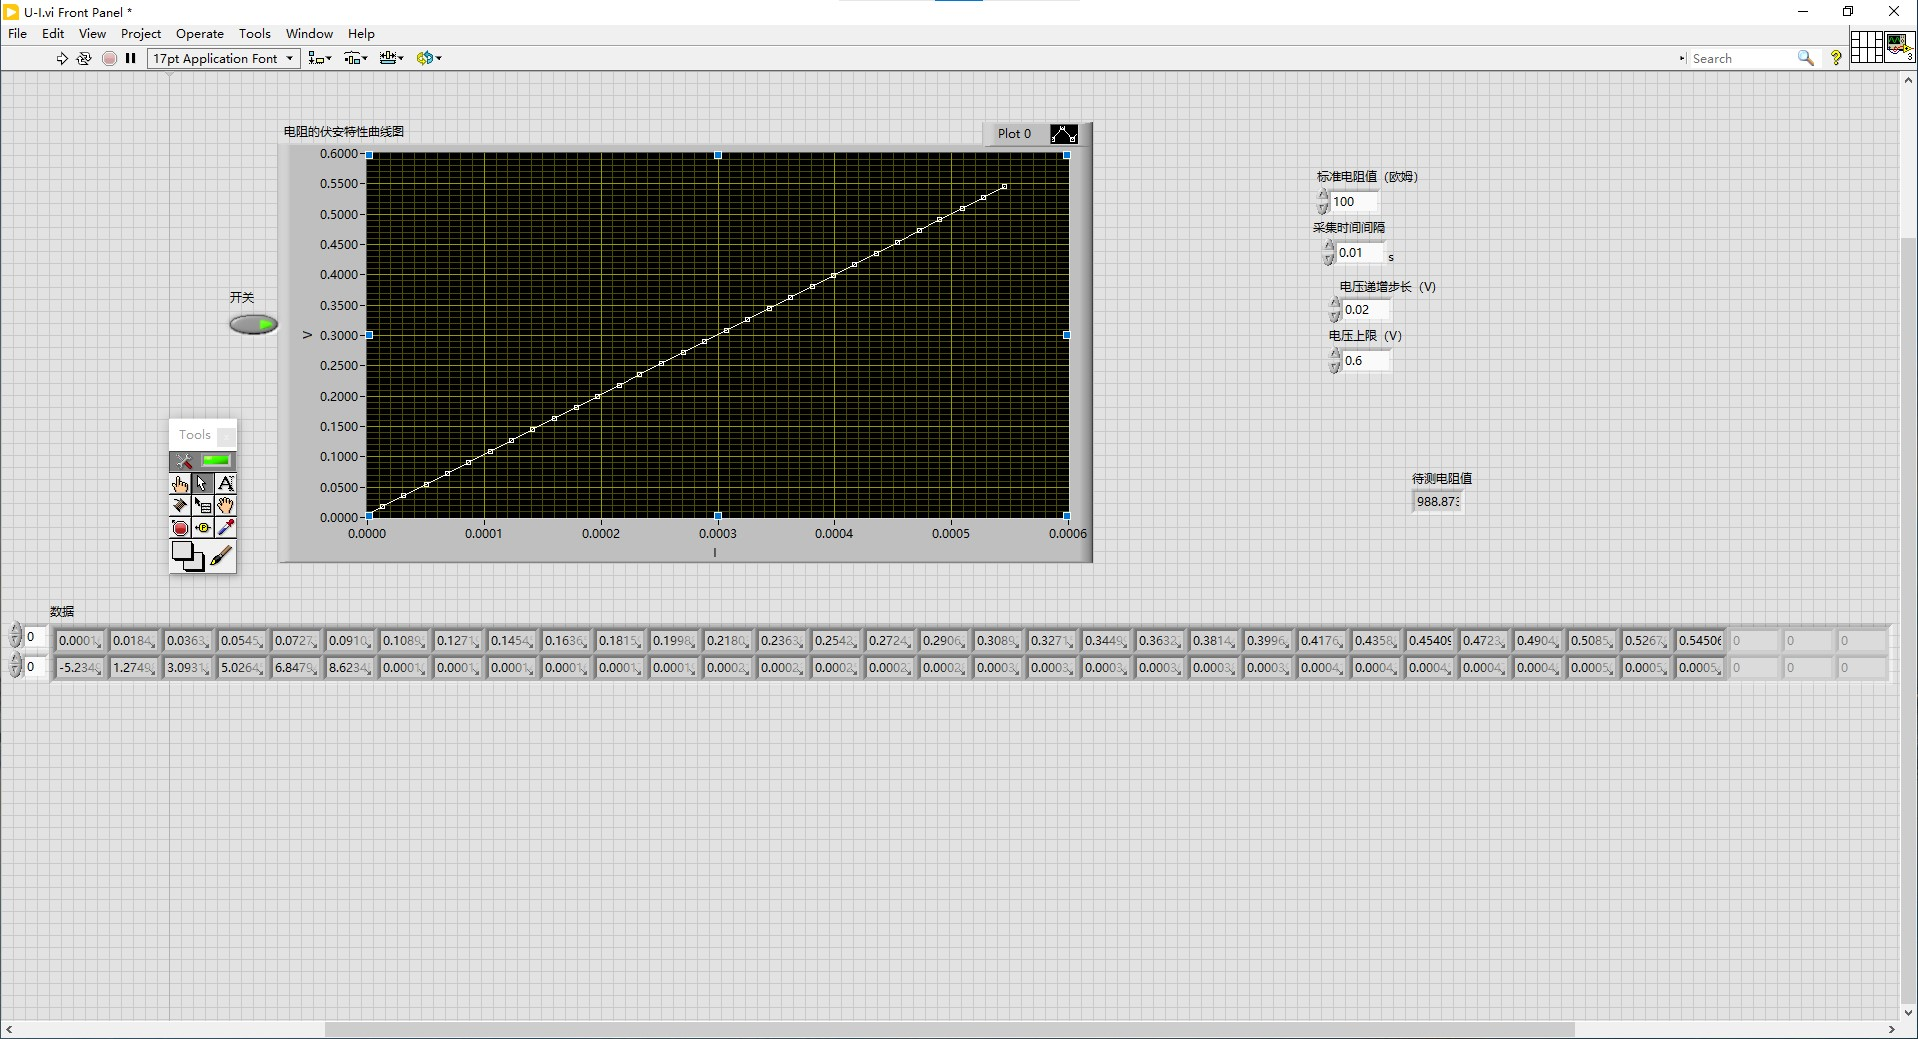
\includegraphics[width=\linewidth]{ui5.jpg}
	\end{figure}
	\begin{figure}[H]
		\centering
		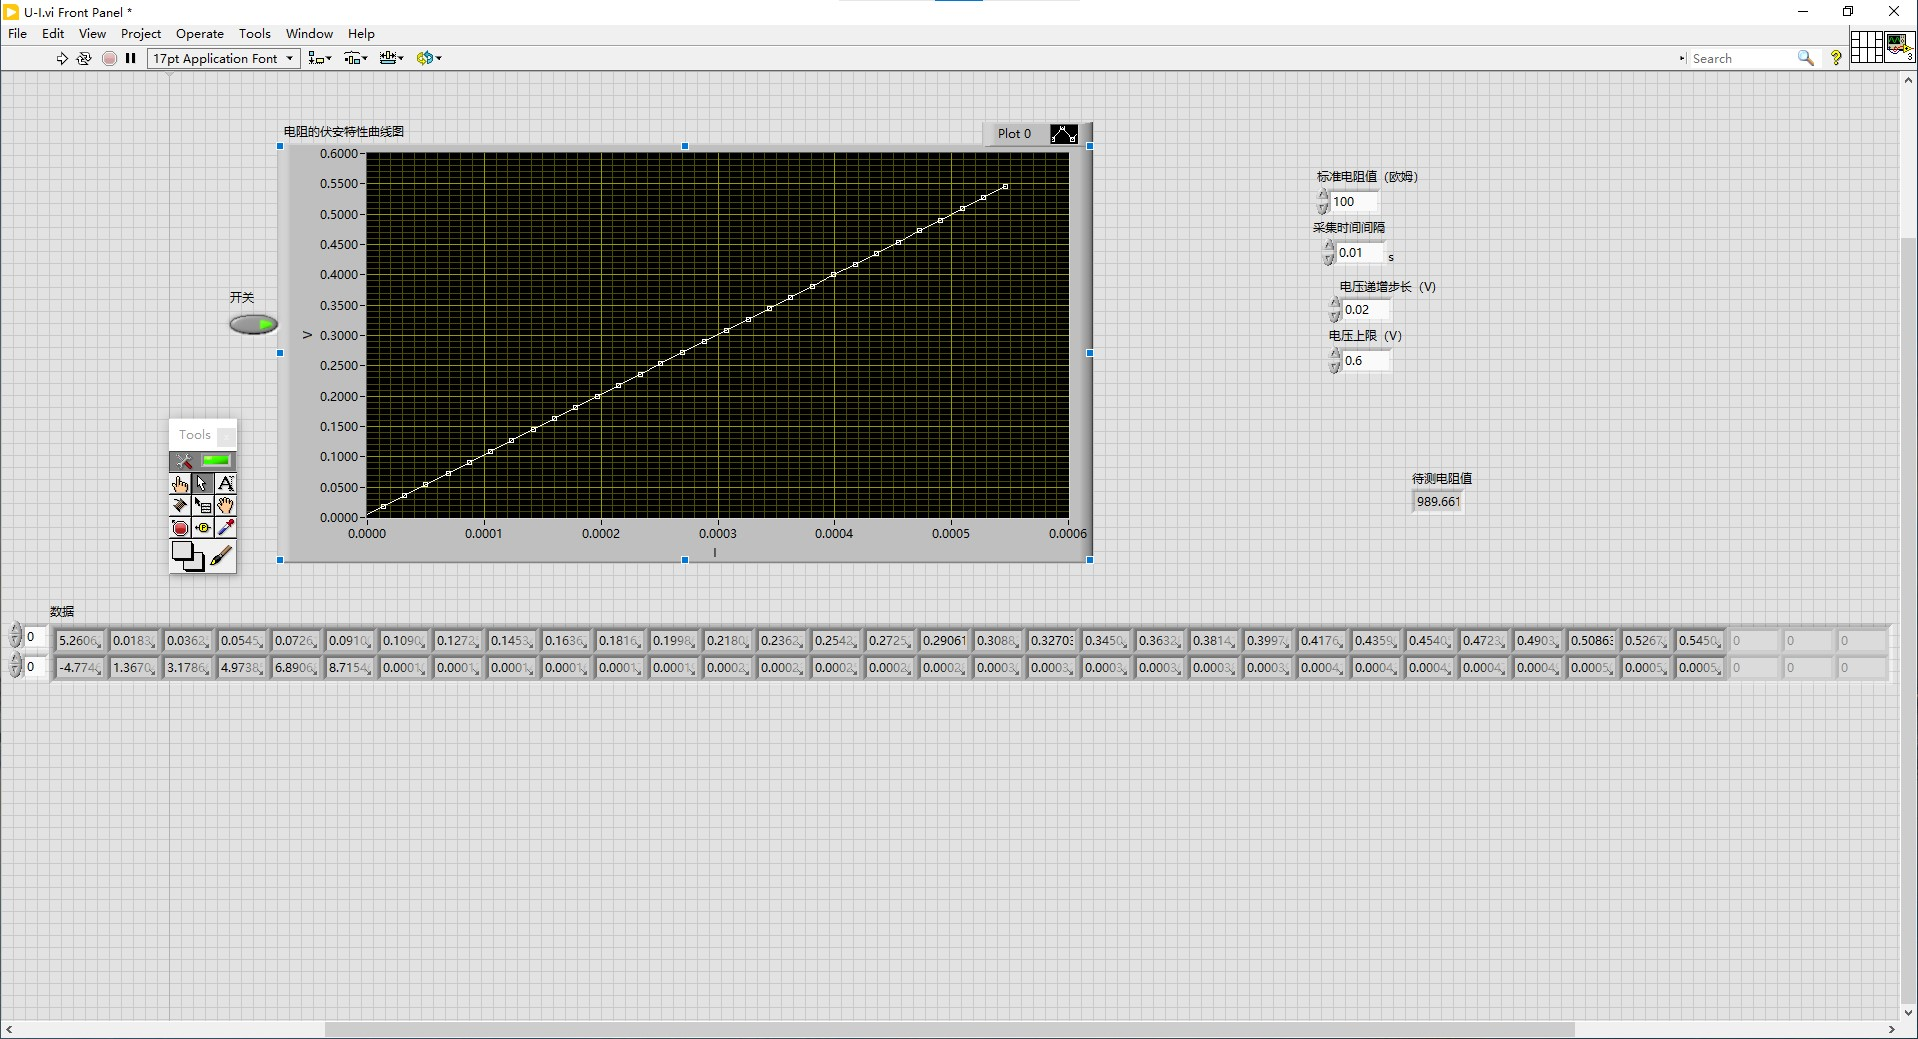
\includegraphics[width=\linewidth]{ui6.jpg}
		\caption{$1000\Omega$电阻测量结果}
	\end{figure}
	分别取三次平均可得
	\begin{align}
		R_1&=51.3608\Omega\\
		R_2&=989.351\Omega
	\end{align}
	\subsection{二极管的正反向伏安特性曲线}
	
	实验测量二极管正反向的伏安特性曲线的方法是分别进行手动测量(均先粗测出大致范围),测量用到的程序框图如图\ref{kuangtu}。
	\begin{figure}[H]
		\centering
		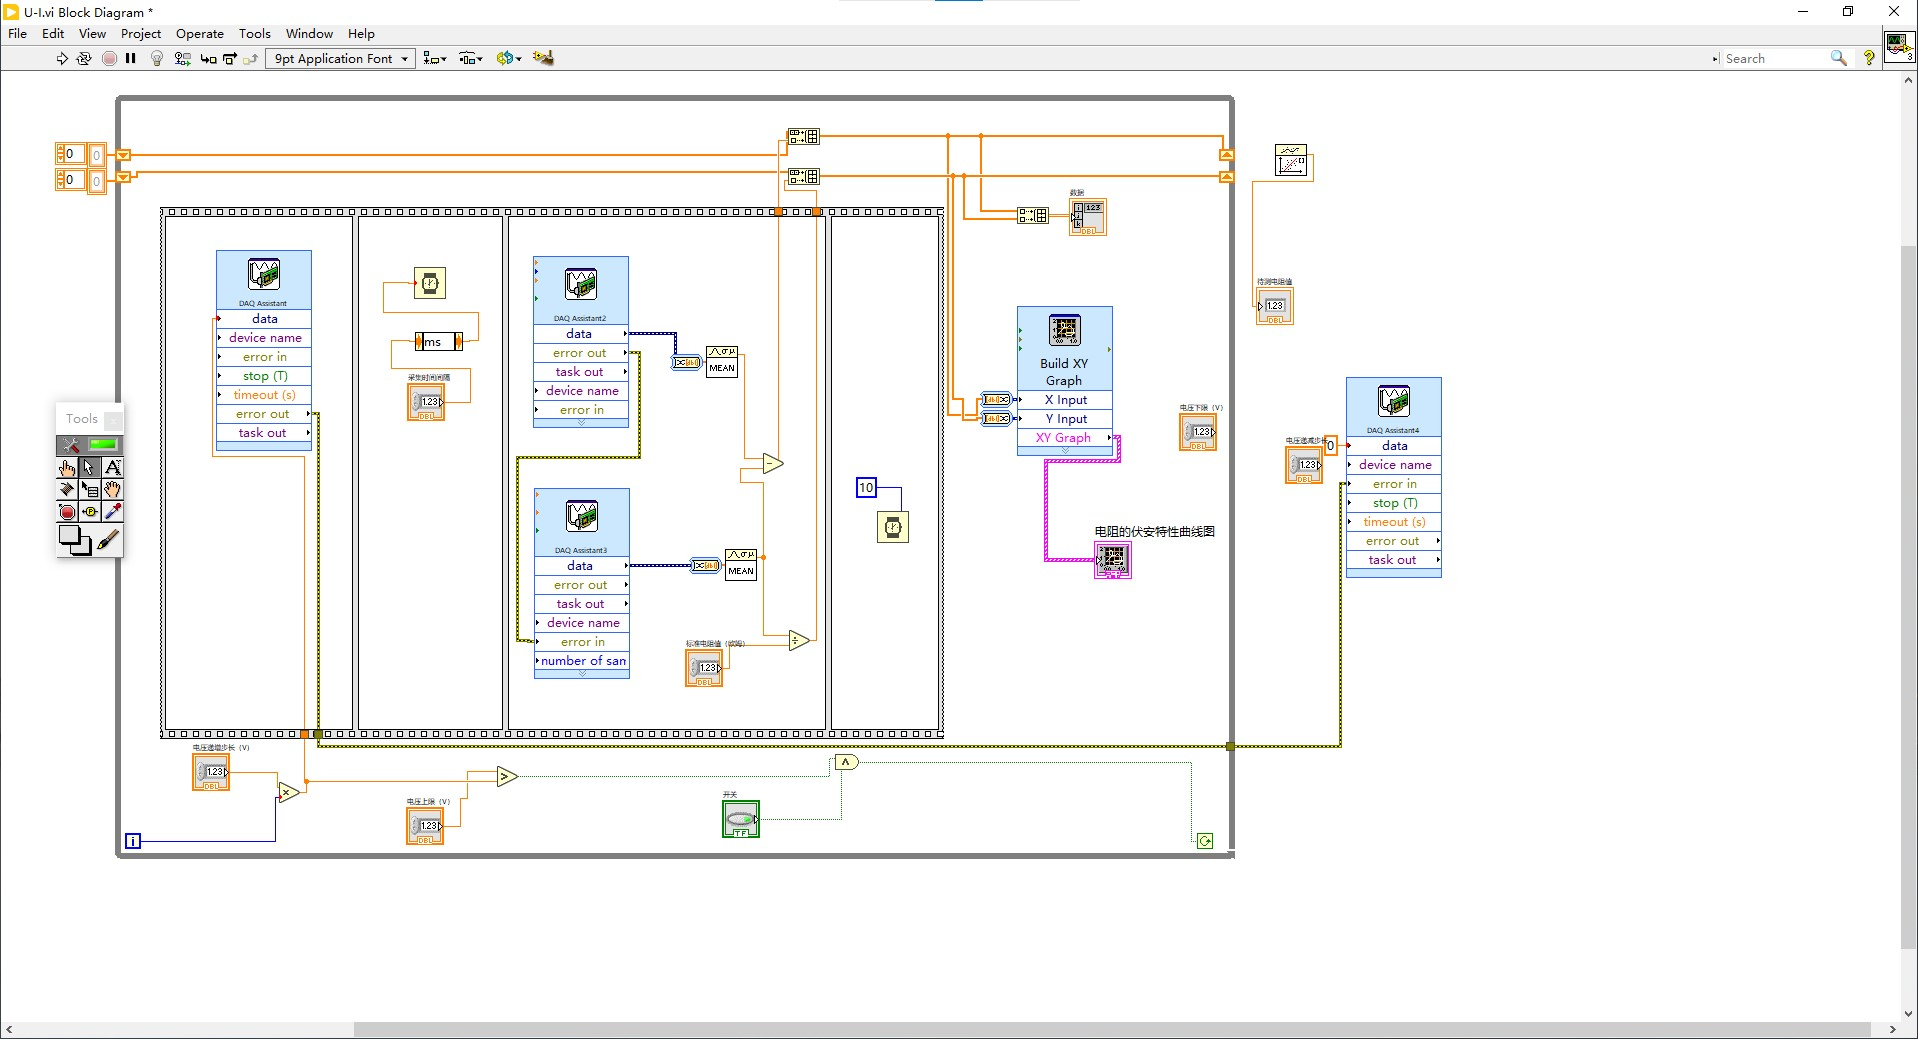
\includegraphics[width=\linewidth]{bi_pro.jpg}
		\caption{测量二极管正反向伏安特性曲线的程序框图}
		\label{kuangtu}
	\end{figure}
	实验测量结果如图\ref{p}、图\ref{n}所示。
	\begin{figure}[H]
		\centering
		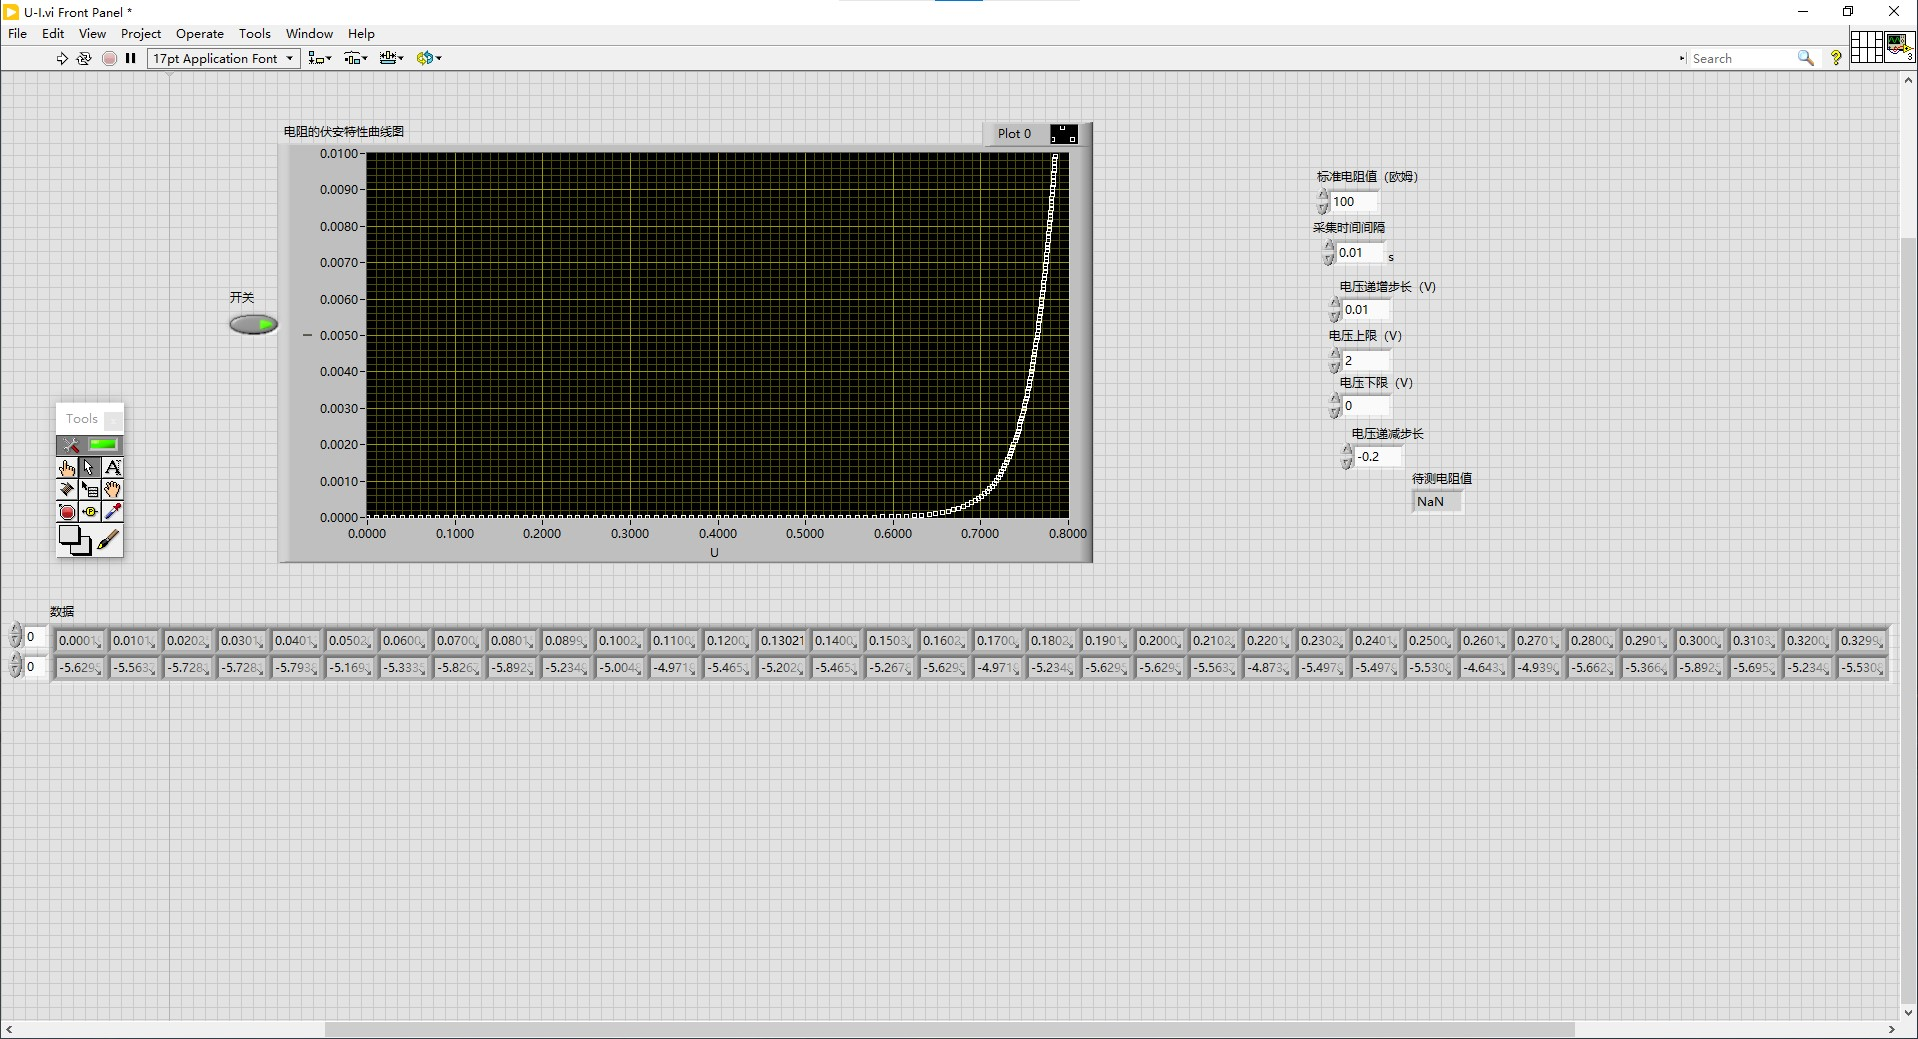
\includegraphics[width=\linewidth]{bi_positive.jpg}
		\caption{二极管正向伏安特性曲线}
		\label{p}
	\end{figure}
	\begin{figure}[H]
		\centering
		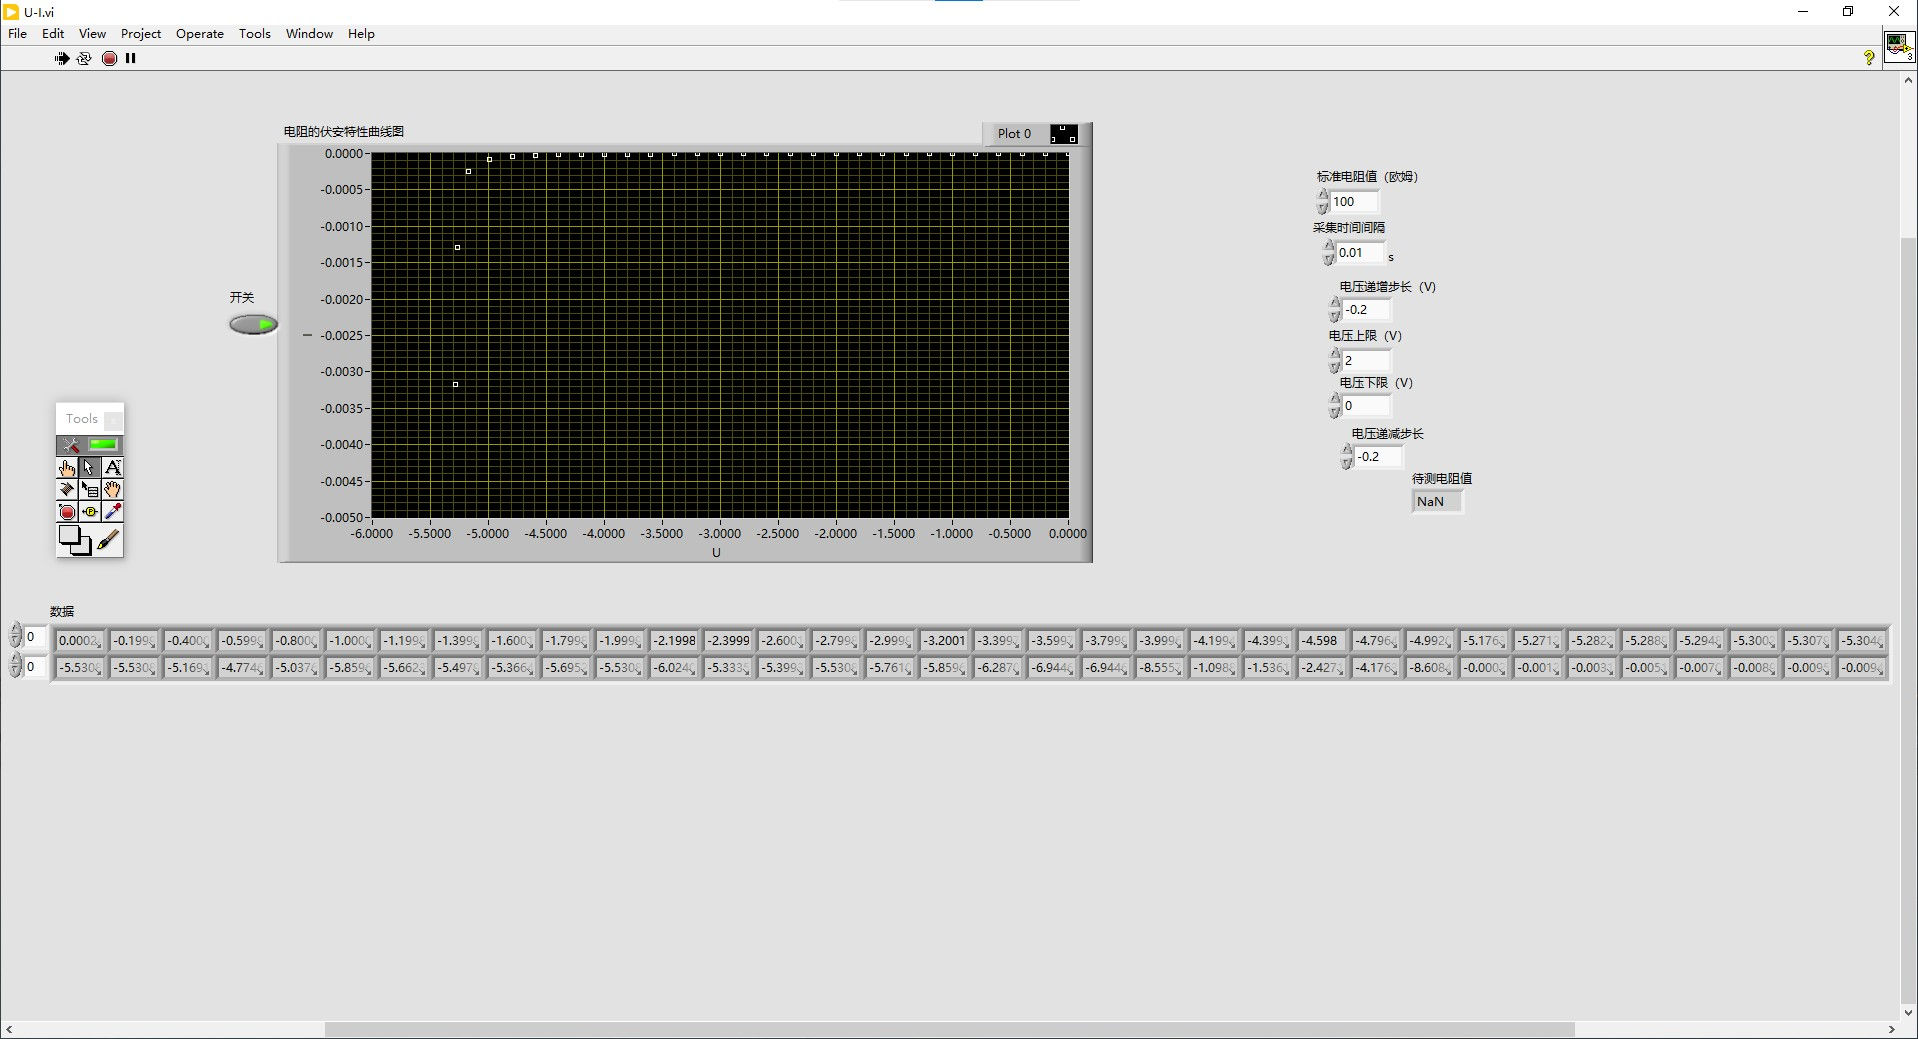
\includegraphics[width=\linewidth]{bi_neg.jpg}
		\caption{二极管反向伏安特性曲线}
		\label{n}
	\end{figure}
	电流为正$4\mathrm{mA}$附近的静态电阻值为
	\begin{align}
		R_{\text{postive}}=\frac{0.76\mathrm{V}}{0.004\mathrm{A}}=190\Omega
	\end{align}
	电流为负$4\mathrm{mA}$附近的静态电阻值为
	\begin{align}
		R_{\text{negative}}=\frac{5.3\mathrm{V}}{0.004\mathrm{A}}=1.32\times10^3\Omega
	\end{align}
	\section{第二次课}
	\subsection{电容电感表征测量}
	该部分主要实验内容为定值电容、电感在不同频率下阻抗等的测量,测量结果如图所示。
	\begin{figure}[H]
		\centering
		\subfigure[电感-频率曲线]{\includegraphics[width=0.4\linewidth]{L18mH_R100Ohm_L.png}}
		\subfigure[耗散电阻-频率曲线]{\includegraphics[width=0.4\linewidth]{L18mH_R100Ohm_Rloss.png}}
	\end{figure}
	\begin{figure}[H]
		\centering
		\subfigure[阻抗-频率曲线]{\includegraphics[width=0.4\linewidth]{L18mH_R100Ohm_Rimpedance.png}}
		\subfigure[相位-频率曲线]{\includegraphics[width=0.4\linewidth]{L18mH_R100Ohm_phase.png}}
		\caption{$18\mathrm{mH}$电感测量结果}
	\end{figure}
	\begin{figure}[H]
		\centering
		\subfigure[电容-频率曲线]{\includegraphics[width=0.4\linewidth]{C0.22uF_R100Ohm_C.png}}
		\subfigure[耗散电阻-频率曲线]{\includegraphics[width=0.4\linewidth]{C0.22uF_R100Ohm_Rloss.png}}
	\end{figure}
	\begin{figure}[H]
		\centering
		\subfigure[阻抗-频率曲线]{\includegraphics[width=0.4\linewidth]{C0.22uF_R100Ohm_Rimpedance.png}}
		\subfigure[相位-频率曲线]{\includegraphics[width=0.4\linewidth]{C0.22uF_R100Ohm_phase.png}}
		\caption{$0.22\mathrm{\mu F}$电容测量结果}
	\end{figure}
	\begin{figure}[H]
		\centering
		\subfigure[电容-频率曲线]{\includegraphics[width=0.4\linewidth]{C0.047uF_R100Ohm_C.png}}
		\subfigure[耗散电阻-频率曲线]{\includegraphics[width=0.4\linewidth]{C0.047uF_R100Ohm_Rloss.png}}
	\end{figure}
	\begin{figure}[H]
		\centering
		\subfigure[阻抗-频率曲线]{\includegraphics[width=0.4\linewidth]{C0.047uF_R100Ohm_Rimpedance.png}}
		\subfigure[相位-频率曲线]{\includegraphics[width=0.4\linewidth]{C0.047uF_R100Ohm_phase.png}}
		\caption{$0.047\mathrm{\mu F}$电容测量结果}
	\end{figure}
	\subsection{Fano线型的探究}
	采用图\ref{circuit}连接电路。取$L_1=18\mathrm{mH},L_2=16\mathrm{mH},C_1=0.047\mathrm{\mu F},C_2=0.2\mathrm{\mu F},C=0.5\mathrm{\mu F},R=500\Omega$。
	\begin{figure}[H]
		\centering
		\includegraphics[width=12cm]{circuit.png}
		\caption{电路示意图}
		\label{circuit}
	\end{figure}
	\subsubsection{实验结果}
	采取上述参数的设定值,可以得到结果曲线如下。
	\begin{figure}[H]
		\centering
		\subfigure[$\frac{I}{U_x}-f$关系图]{\includegraphics[width=10cm]{standard.png}
			\label{fano}}\\
		\subfigure[$(\varphi_I-\varphi_x)-f$关系图]{\includegraphics[width=10cm]{standard_phase.png}
			\label{fanophase}}
		\caption{Fano线型的观测}
	\end{figure}
	可见,我们成功的观察到了Fano共振的非对称特征,可以发现,其响应谱更加陡峭、更加尖锐。
	\subsubsection{对一些参数的改变}
	\paragraph{对$C_2$的改变}
	改变$C_2$的值依次为$0.1\mathrm{\mu F},0.08\mathrm{\mu F},0.07\mathrm{\mu F},0.06\mathrm{\mu F},0.05\mathrm{\mu F},0.04\mathrm{\mu F},0.03\mathrm{\mu F}$,均测量$\frac{I}{U_x}-f$和$(\varphi_I-\varphi_x)-f$曲线并绘制在一张图中,可得图\ref{comparison}、图\ref{comparison_phase}。
	\begin{figure}[H]
		\centering
		\subfigure[$\frac{I}{U_x}-f$关系图]{\includegraphics[width=10cm]{c2_comparison.png}
			\label{comparison}}
		\\
		\subfigure[$(\varphi_I-\varphi_x)-f$关系图]{\includegraphics[width=10cm]{c2_comparison_phase.png}
			\label{comparison_phase}}
		\caption{改变$C_2$后Fano线型的对比图}
	\end{figure}
	\paragraph{对$R$的改变}
	改变$R$分别为$100\Omega,2000\Omega$\footnote{由于时间原因,并没有足够的时间多次改变$C$的值并进行测量},得到图\ref{Rcomparison}、图\ref{Rcomparison_phase}
	\begin{figure}[H]
		\centering
		\subfigure[$\frac{I}{U_x}-f$关系图]{\includegraphics[width=10cm]{R_comparison.png}
			\label{Rcomparison}}\\
		\subfigure[$(\varphi_I-\varphi_x)-f$关系图]{\includegraphics[width=10cm]{R_comparison_phase.png}
			\label{Rcomparison_phase}}
		\caption{改变$R$后Fano线型的对比图}
	\end{figure}
	\paragraph{对$C$的改变}
	改变共用电容$C$分别为$0.05\mathrm{\mu F},1\mathrm{\mu F}$\footnote{由于时间原因,并没有足够的时间多次改变$R$的值并进行测量},得到图\ref{Ccomparison}、图\ref{Ccomparison_phase}
	\begin{figure}[H]
		\centering
		\subfigure[$\frac{I}{U_x}-f$关系图]{\includegraphics[width=10cm]{C_comparison.png}
			\label{Ccomparison}}\\
		\subfigure[$(\varphi_I-\varphi_x)-f$关系图]{\includegraphics[width=10cm]{C_comparison_phase.png}
			\label{Ccomparison_phase}}
		\caption{改变$C$后Fano线型的对比图}
	\end{figure}
	\subsubsection{对结果的分析}
	\paragraph{关于Fano线型}
	根据图\ref{circuit}给出的电路,我们可以很轻松地得到
	\begin{align}
		\omega_1^2=\frac{1}{L_1}(\frac{1}{C_1}+\frac{1}{C})&,\omega_2^2=\frac{1}{L_2}(\frac{1}{C_2}+\frac{1}{C})\label{eq:omega}\\
		\gamma_1=\frac{R}{L_1},\gamma_2=\frac{R}{L_2}&,g^2=\frac{1}{C^2L_1L_2}\label{eq:gamma}
	\end{align}
	带入初始给出的数值,可以计算出两个子回路的本征频率
	\begin{align}
		f_1=5.7\times10^3\mathrm{Hz},f_2=3.3\times10^3\mathrm{Hz}
	\end{align}
	可以看到图\ref{fano}以及图\ref{fanophase}中的比较特殊的曲线段就在$f_1,f_2$附近,这也就说明了Fano线型是两个振荡系统相互耦合得到的(也可成为干涉)。图\ref{fano}中的窄峰可以理解为干涉效应导致某些频率下的相应被加强,而其它频率则因为干涉相消而减弱,而宽峰就是正常的幅频特性。这也可以通过相频特性看出(图\ref{fanophase})。
	\paragraph{对$C_2$的改变}
	对$C_2$的改变是在几个改变参数中最有效的,这是因为调节$C_2$只会影响$\omega_2$(及$f_2$)的变化,相当于保持$f_1$主峰不动,然后另外一个变化,这有助于控制变量,方便的观察其它条件不变时,在原来振荡系统上耦合的振荡系统的变化对整体造成的影响。
	
	当$C_2$变小,对应的$f_2$变大,会导致Fano线型的右移,并在$C_2\approx0.05\mathrm{\mu F}$时形成一个近似对称的分布(Quasi-Lorentz线型),之后Fano线型位于主峰的右侧。
	
	同时,还可以注意到随着$C_2$的变小,Fano线型的上顶点有一个先变大后变小的趋势,且最大值不会超过主峰。这可能是电容变化、频率变化导致的复阻抗的变化造成的。
	\paragraph{对$R$的改变}
	调节$R$的值是非常没用的,根据式\ref{eq:omega}和式\ref{eq:gamma},$R$的改变只会影响$\gamma_1,\gamma_2$,即曲线的幅度会有变化,当$R$变大,系统的损耗变大,所以所得到的曲线幅度变小,如图\ref{Rcomparison}所示,而相位为零对应的频率值、以及峰所对应的频率值都不会发生改变,如图\ref{Rcomparison}、图\ref{Rcomparison_phase}所示。图\ref{Rcomparison_phase}中三条曲线交于一点就是因为改变电阻值不会影响谐振($\varphi_I-\varphi_x=0$时)的频率。
	\paragraph{对$C$的改变}
	对$C$的改变会同时影响$f_1$和$f_2$,所以曲线的变化关系会比较混乱\footnote{尤其是只有三条曲线且$C$的取值并不是非常合理的时候,显然,实验过程中$C$改变的取值很不合理}。由于$C$变大,$f_1$和$f_2$都变小,两个峰都向左移,如图\ref{Ccomparison}、图\ref{Ccomparison_phase}所示。
\end{document}